\documentclass{article}
%Reporte de computacional
\usepackage{hyperref}
\usepackage{amsmath}
\usepackage{amsthm}
\usepackage{amssymb}
\usepackage{graphicx}
\usepackage{ifxetex}
\ifxetex
\usepackage{fontspec}
\else
\usepackage[T1]{fontenc}
\usepackage[utf8]{inputec}
\usepackage{lmodern}
\fi


\begin{document}
\title{Preparando Datos Con Emacs}
\author{Ramses Pacheco Ortiz}
\date{6 De marzo Del 2018}
\maketitle  


\section{Introduccion}

Esta sección es un curso intensivo sobre el editor de textos emacs, en donde la actividad anterior lo utilizamos para descargar unos datos de sondeos y para la realización de los scripts,en esta ocacion utilizaremos emacs para editar el archivo de datos decargados en la actividad anterior(Introducción a la programación de los intérpretes de comandos),cambiandole las fechas por numeros de mes ,modificando los espacios,etc.


Emacs es un editor de texto con una gran cantidad de funciones, muy popular entre programadores y usuarios técnicos. GNU Emacs es parte del proyecto GNU y la versión más popular de Emacs con una gran actividad en su desarrollo.
El Emacs original significa, \textbf{E}ditor \textbf{MAC}ro\textbf{S }para el TECO. Fue escrito en 1975 por Richard Stallman junto con Guy Steele. Fue inspirado por las ideas de TECMAC y TMACS, un par de editores TECO-macro escritos por Guy Steele, Dave Moon, Richard Greenblatt y otros. Se han lanzado muchas versiones de EMACS hasta el momento, pero actualmente hay dos que son usadas comúnmente: 

\textbf{GNU Emacs}, iniciado por Richard Stallman en 1984, y \textbf{XEmacs}, una fork de GNU Emacs, que fue iniciado en 1991. Ambos usan una extensión de lenguaje muy poderosa, Emacs Lisp, que permite manejar tareas distintas, desde escribir y compilar programas hasta navegar en Internet. GNU Emacs es mantenido por el Proyecto GNU Emacs, el cual cuenta entre sus miembros a Richard Stallman.


\section{Conceptos CAPE y PW}
\begin{itemize}
\item CAPE

Uno de los problemas en la estimación de la inestabilidad atmosférica (uno de los ingredientes necesarios para el desarrollo de la convección, junto con la humedad y mecanismo de disparo que inicie el ascenso de la masa de aire) es su cuantificación y su aplicabilidad en la realidad diaria. Para poder llegar a este punto vamos a presentar uno de los índices más populares y usados para tal fin, la CAPE (Convective Available Potencial Energy, en inglés) o energía potencial disponible convectiva.  La CAPE se mide en Julios por kilogramos, J/kg, y estrictamente hablando no es un índice de inestabilidad propiamente dicho como otros índices más clásicos.

a CAPE representa la cantidad de energía de flotabilidad disponible de una parcela o burbuja de aire  que se eleva vertical y libremente” o “la cantidad de  trabajo que una burbuja o parcela de aire hace en el medio ambiente al ascender libremente”.

\item{PW}
La distribución y evolución del vapor de agua es determinante en el funcionamiento climático y meteorológico de la atmosfera terrestre. Hasta hace poco tiempo, esta variable atmosférica no estaba bien definida al no disponerse de medidas con la suficiente resolución para representar su alta inestabilidad espacial y temporal. El incremento en los últimos años de estaciones de referencia permanentes GNSS a escala mundial, supone un importante avance para la monitorización del vapor de agua o cantidad de \textbf{agua precipitable} (PW). El objetivo de esta Tesis es analizar el comportamiento del contenido de vapor de agua atmosférico determinado a partir de las observaciones GNSS realizadas en las estaciones de referencia localizadas en la Comunidad Valenciana, estableciendo un sistema de observación y monitorización atmosférica en la zona de estudio, donde se han establecido las relaciones del PW con las variables meteorológicas presión atmosférica y precipitación, evaluando la tendencia y variabilidad del vapor de agua atmosférico cuando se han sucedido eventos de lluvias intensas.

\section{Descripcion Del Proceso De Limpieza Y Preparacion De Los Datos}

Anteriormente a esta actividad descargamos unos datos de un pais de nuestra eleccion,unas de las clasificaciones que tienen estos datos son la
temperatura, presion, altura, humedad, velocidad en nudos,etc.

\vspace{1mm}
Con ayuda de emacs modificaremos el archivo antes mencionado, eliminando clasificaciones y dejando solamente 2  las cuales llevan el nombre de CAPE Y PW,los cuales lo guardamos en otro archivo llamado df2017CAPE\_PW.csv
A continuacion se le muestra el codigo con el cual se llevo la accion mencionada:


\begin{center}
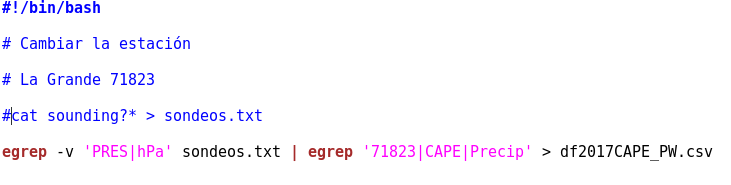
\includegraphics[height=5cm]{act5.png}
\end{center}



Despues creamos otros dos archivos a partir del archivo creado anteriormente, llamandolos a uno de ellos como df2017CAPE\_PW\_00Z.csv y otro df2017CAPE\_PW\_12Z.csv, en la siguiennte imagen muestra como los creamos y los datos de los archivos:

\begin{center}
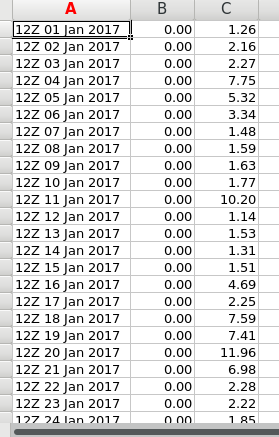
\includegraphics[height=8cm]{act512z.png}
\end{center}

\begin{center}
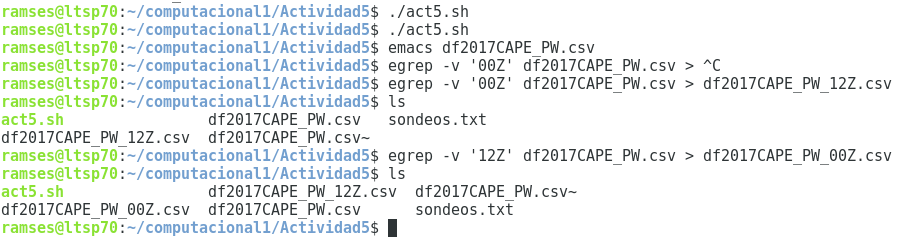
\includegraphics[height=4cm]{act5_3.png}
\end{center}

\vspace{0.5mm}

Ya que obtuvimos el archivo con los datos necesarios, lo abrimos con la aplicacion emacs para hacer las modificaciones, unas de las modificaciones es eliminar el 12z y el jan cambiarlo con numero respecto al mes por ejemplo en este caso del jan seria (01).para llevar acabo esto utilizamos unos comando para seleccionar la palabra comun que queremos cambiar y despues remplazando el numero correspondiente al mes, la imagen siguiente muestra el resultado final.

\begin{center}
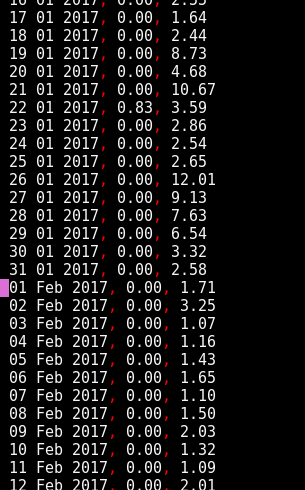
\includegraphics[height=8cm]{act5_2.png}
\end{center}


\begin{center}
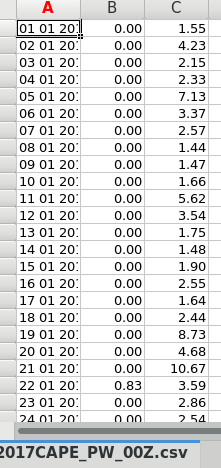
\includegraphics[height=8cm]{act00z.png}
\end{center}

\vspace{1mm}

ahora que obtuvimos los dos archivos separados,sin mes por escritro y con las modificacion realizadas anteriormente procederemos a pasarlas a la libreria pandas para posteriormente leer los archivos,en la siguiente imagen se muestra el codigo utilizado.

\begin{center}
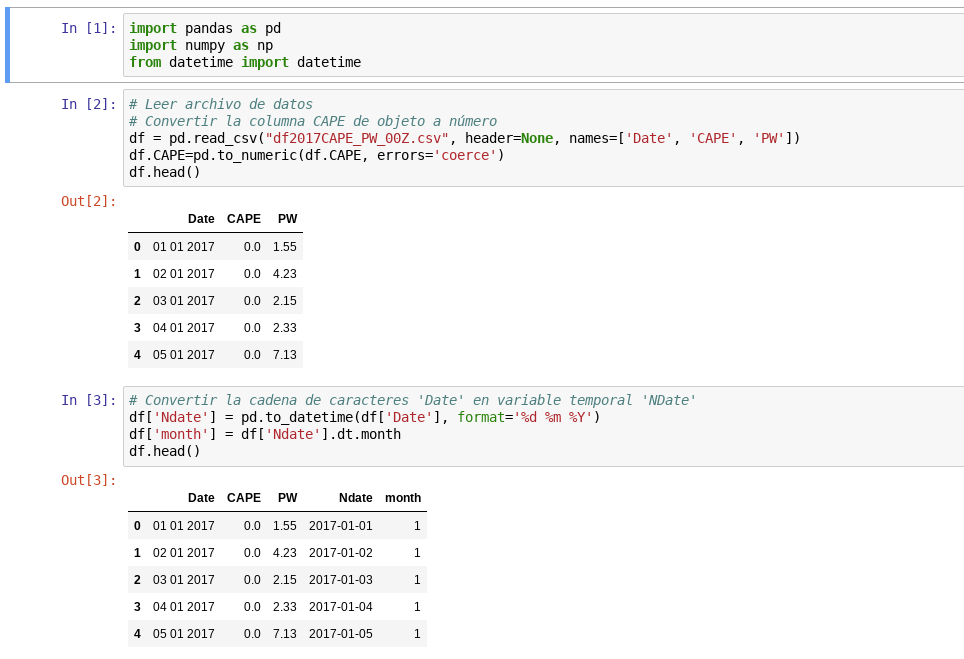
\includegraphics[height=8cm]{jupyter.png}
\end{center}

Ya que leeimos los datos que hibamos a utilizar y los caracteres necesarios,proseguiremos a realizar una boxplot con los datos, acontinuacion se muestra la grafica de caja de los dos meses mostrados junio y diciembre:

\begin{center}
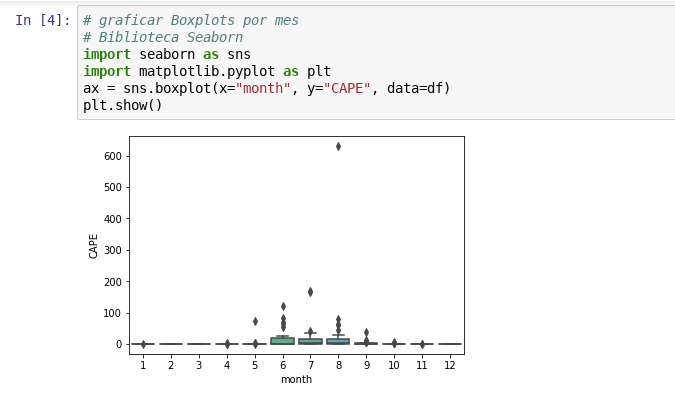
\includegraphics[height=8cm]{jupyter1.png}
\end{center}

\begin{center}
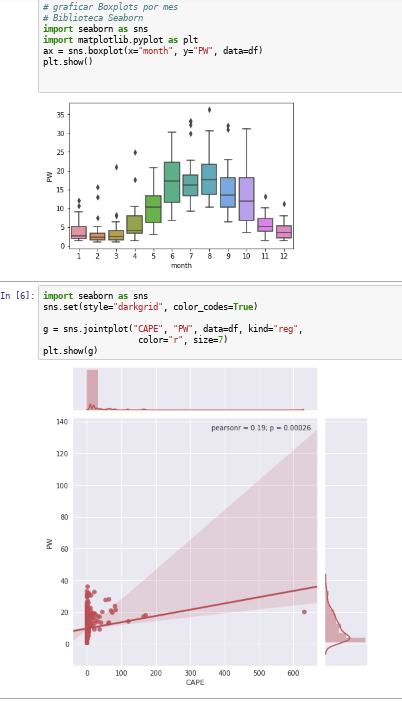
\includegraphics[height=10cm]{jupyter3.png}
\end{center}


por ultimo mostramos una grafica mas gradual del mes:

\begin{center}
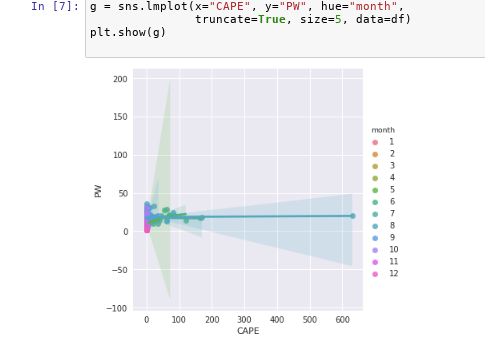
\includegraphics[height=8cm]{jupyter4.png}
\end{center}




\end{itemize}

\section{Conclusiones}

Me paracio mu interesante esta practica ya que aprendimos mas sobre emacs y como editar textos, nos mostro como es una herramienta muy util y conocimos ciertos comando que nos facilitara el uso de este editor cuando tengamos muchos datos.

por otro lado aprendimos algo nuevo en python, algo que nunca habiamos visto que son las graficas de caja, me paracio muy interesante aunque, no busque informacion mas a fondo sobre estas graficas.



\section{Bibliografia}

\begin{itemize}
\item Curso sobre interpretación de mapas meteorológicos: la CAPE (Convective Available Potencial Energy) - Revista del Aficionado a la Meteorología. (2018). Revista del Aficionado a la Meteorología.https://www.tiempo.com/ram/800/curso-sobre-interpretacin-de-mapas-meteorolgicos-el-cape-convective-available-potencial-energy/

\item
Emacs. (2018). Es.wikipedia.org. https://es.wikipedia.org/wiki/Emacs

\item

antos, J. (2018). Análisis y predicción de lluvias intensas en la Comunidad Valenciana basados en la estimación del contenido de vapor de agua atmosférico obtenido con técnicas GNSS. Dialnet.unirioja.es.https://dialnet.unirioja.es/servlet/tesis



\section{Apéndice}

\textbf{¿Cómo se te hizo esta actividad? ¿Compleja, Difícil, Sencilla?}

Un poco dificil y confusa , ya que estudiamos algo nuevo que nunca habiamos realizado practicamente

\textbf{¿Qué te llamó más la atención?}

Me llamo mucho la atencion las graficas de caja y el editor de emacs, como nos facilitara la vida.
\textbf{¿Qué parte fue la que menos te interesó hacer?}

ninguna


\textbf{¿Cómo mejorarías esta actividad? ¿Qué le faltó? ¿Qué sobró?}

Talvez con un poco mas de instrucciones en las actividades a realizar.

\textbf{¿Hasta este punto, que te parece el uso de Jupyter para programar en Python? 
 }
 
 Bien, la plataforma es como para trabajar y facil de comprender.


\end{itemize}




\end{document}

